\captionsetup{justification=centering,margin=0cm}
\label{cap:atividade3}  % Forma de referenciar o capítulo no comando \ref

%inicio do capitulo
\chapter[Atividade 3: O DESEMPENHO DO PNG-24 EM IMAGENS COM DIFERENTES CONTEÚDOS]{Atividade 3: O DESEMPENHO DO PNG-24 EM IMAGENS COM DIFERENTES CONTEÚDOS}

Agora que avaliamos empiricamente as imagens, é chegado o momento de averiguar a qualidade do método\footnote{Em momento algum dissemos que ele era bom ou confiável.}. Para tal, primeiro comprimiu-se cada imagem em formato formato sem perdas utilizando os \textit{softwares} \textit{WinRar} e \textit{PNG-24}. Todos os resultados estão descritos na Tabela \ref{tab:compressão_sem_perdas}. Por questões de formatação dessa tabela gigante, vamos continuar o texto na página 21. 

\begin{table}[htbp]
\centering

\caption{Resultados das Compressões sem Perdas.}
\label{tab:compressão_sem_perdas}

\scriptsize

\begin{tabularx}{\textwidth}{X|C|C|C|C|C|C|C|C}
    \hline
        
        \multirow{2}{*}{\textbf{Imagem}} & \multirow{2}{*}{\textbf{\makecell{Tamanho \\ Original}}} & \multicolumn{2}{c|}{\textbf{RAR}} & \multicolumn{2}{c|}{\textbf{ZIP}} & \multicolumn{2}{c|}{\textbf{PNG-24}} & \textbf{\multirow{2}{*}{\makecell{Comple-\\xidade}}} \\ \hhline{~~------~}
        ~ & ~ & \textbf{Tamanho} & \textbf{Ratio} & \textbf{Tamanho} & \textbf{Ratio} & \textbf{Tamanho} & \textbf{Ratio} & ~ \\ \hline
IMG01 & 4.320.056 & 1.682.160 & 0,39 & 1.792.289 & 0,41 & 1.613.669 & 0,37 & MÉDIA BAIXA \\ \hline
        IMG02 & 4.320.056 & 2.456.915 & 0,57 & 3.084.276 & 0,71 & 2.126.163 & 0,49 & MÉDIA BAIXA \\ \hline
        IMG03 & 4.320.056 & 1.152.309 & 0,27 & 1.207.949 & 0,28 & 1.042.306 & 0,24 & BAIXA \\ \hline
        IMG04 & 4.320.056 & 2.182.793 & 0,51 & 2.470.507 & 0,57 & 1.822.802 & 0,42 & MÉDIA BAIXA \\ \hline
        IMG05 & 4.320.056 & 2.127.441 & 0,49 & 2.738.041 & 0,63 & 1.885.248 & 0,44 & MÉDIA BAIXA \\ \hline
        IMG06 & 4.320.056 & 2.135.632 & 0,49 & 2.895.875 & 0,67 & 1.915.684 & 0,44 & MÉDIA BAIXA \\ \hline
        IMG07 & 4.320.056 & 1.818.370 & 0,42 & 2.204.978 & 0,51 & 1.572.060 & 0,36 & MÉDIA BAIXA \\ \hline
        IMG08 & 4.320.056 & 4.104.336 & 0,95 & 4.151.487 & 0,96 & 3.513.270 & 0,81 & ALTA \\ \hline
        IMG09 & 4.320.056 & 2.218.660 & 0,51 & 2.689.768 & 0,62 & 1.960.195 & 0,45 & MÉDIA BAIXA \\ \hline
        IMG10 & 4.320.056 & 2.877.708 & 0,67 & 3.369.460 & 0,78 & 2.509.826 & 0,58 & MÉDIA ALTA \\ \hline
        IMG11 & 4.320.056 & 3.791.085 & 0,88 & 3.941.896 & 0,91 & 3.224.670 & 0,75 & ALTA \\ \hline
        IMG12 & 4.320.056 & 3.242.145 & 0,75 & 3.682.728 & 0,85 & 2.569.986 & 0,59 & MÉDIA ALTA \\ \hline
        IMG13 & 4.320.056 & 2.929.852 & 0,68 & 3.430.984 & 0,79 & 2.568.571 & 0,59 & MÉDIA ALTA \\ \hline
        IMG14 & 4.320.056 & 2.865.353 & 0,66 & 3.696.286 & 0,86 & 2.329.559 & 0,54 & MÉDIA ALTA \\ \hline
        IMG15 & 4.320.056 & 1.252.278 & 0,29 & 1.656.743 & 0,38 & 1.156.266 & 0,27 & BAIXA \\ \hline
        IMG16 & 4.320.056 & 2.801.431 & 0,65 & 3.982.515 & 0,92 & 2.489.280 & 0,58 & MÉDIA ALTA \\ \hline
        IMG17 & 4.320.056 & 2.952.275 & 0,68 & 3.756.000 & 0,87 & 2.466.793 & 0,57 & MÉDIA ALTA \\ \hline
        IMG18 & 4.320.056 & 2.204.070 & 0,51 & 3.611.077 & 0,84 & 1.906.284 & 0,44 & MÉDIA BAIXA \\ \hline
        IMG19 & 4.320.056 & 3.175.453 & 0,74 & 3.813.659 & 0,88 & 2.683.151 & 0,62 & MÉDIA ALTA \\ \hline
        IMG20 & 4.320.056 & 3.343.184 & 0,77 & 3.863.819 & 0,89 & 3.127.814 & 0,72 & ALTA \\ \hline
        IMG21 & 4.320.056 & 1.743.464 & 0,40 & 2.023.594 & 0,47 & 1.582.110 & 0,37 & MÉDIA BAIXA \\ \hline
        IMG22 & 4.320.056 & 3.085.544 & 0,71 & 3.817.534 & 0,88 & 2.649.058 & 0,61 & MÉDIA ALTA \\ \hline
        IMG23 & 4.320.056 & 2.434.239 & 0,56 & 2.897.198 & 0,67 & 2.246.862 & 0,52 & MÉDIA ALTA \\ \hline
        IMG24 & 4.320.056 & 2.421.612 & 0,56 & 2.530.461 & 0,59 & 2.412.455 & 0,56 & MÉDIA ALTA \\ \hline
        IMG25 & 4.320.056 & 2.621.750 & 0,61 & 3.395.123 & 0,79 & 2.287.870 & 0,53 & MÉDIA ALTA \\

    \hline
    
\end{tabularx}

\autoriaPropria

\end{table}

\begin{table}[htbp]
\centering

\small Tabela \ref{tab:compressão_sem_perdas} - Continuação.
\vspace{2 mm}

\scriptsize

\begin{tabularx}{\textwidth}{X|C|C|C|C|C|C|C|C}
    \hline
        
        \multirow{2}{*}{\textbf{Imagem}} & \multirow{2}{*}{\textbf{\makecell{Tamanho \\ Original}}} & \multicolumn{2}{c|}{\textbf{RAR}} & \multicolumn{2}{c|}{\textbf{ZIP}} & \multicolumn{2}{c|}{\textbf{PNG-24}} & \textbf{\multirow{2}{*}{\makecell{Comple-\\xidade}}} \\ \hhline{~~------~}
        ~ & ~ & \textbf{Tamanho} & \textbf{Ratio} & \textbf{Tamanho} & \textbf{Ratio} & \textbf{Tamanho} & \textbf{Ratio} & ~ \\ \hline
        IMG25 & 4.320.056 & 2.621.750 & 0,61 & 3.395.123 & 0,79 & 2.287.870 & 0,53 & MÉDIA ALTA \\ \hline
        IMG26 & 4.320.056 & 1.632.714 & 0,38 & 2.283.075 & 0,53 & 1.676.966 & 0,39 & MÉDIA BAIXA \\ \hline
        IMG27 & 4.320.056 & 3.629.168 & 0,84 & 4.038.880 & 0,93 & 3.220.560 & 0,75 & ALTA \\ \hline
        IMG28 & 4.320.056 & 2.942.101 & 0,68 & 3.366.239 & 0,78 & 2.325.051 & 0,54 & MÉDIA ALTA \\ \hline
        IMG29 & 4.320.056 & 832.501 & 0,19 & 1.083.887 & 0,25 & 692.210 & 0,16 & BAIXA \\ \hline
        IMG30 & 4.320.056 & 1.699.676 & 0,39 & 2.202.509 & 0,51 & 1.445.622 & 0,33 & BAIXA \\ \hline
        IMG31 & 4.320.056 & 2.342.786 & 0,54 & 2.426.433 & 0,56 & 1.881.345 & 0,44 & MÉDIA BAIXA \\ \hline
        IMG32 & 4.320.056 & 2.885.717 & 0,67 & 3.310.647 & 0,77 & 2.533.661 & 0,59 & MÉDIA ALTA \\ \hline
        IMG33 & 4.320.056 & 3.365.152 & 0,78 & 3.681.483 & 0,85 & 2.956.042 & 0,68 & MÉDIA ALTA \\ \hline
        IMG34 & 4.320.056 & 2.419.475 & 0,56 & 3.307.563 & 0,77 & 2.046.515 & 0,47 & MÉDIA BAIXA \\ \hline
        IMG35 & 4.320.056 & 2.802.699 & 0,65 & 3.733.691 & 0,86 & 2.304.984 & 0,53 & MÉDIA ALTA \\ \hline
        IMG36 & 4.320.056 & 1.194.479 & 0,28 & 1.226.554 & 0,28 & 1.092.302 & 0,25 & BAIXA \\ \hline
        IMG37 & 4.320.056 & 3.104.189 & 0,72 & 3.450.910 & 0,80 & 2.822.178 & 0,65 & MÉDIA ALTA \\ \hline
        IMG38 & 4.320.056 & 3.430.765 & 0,79 & 3.894.082 & 0,90 & 3.048.615 & 0,71 & ALTA \\ \hline
        IMG39 & 4.320.056 & 2.926.763 & 0,68 & 3.276.377 & 0,76 & 2.564.862 & 0,59 & MÉDIA ALTA \\ \hline
        IMG40 & 4.320.056 & 2.771.836 & 0,64 & 3.359.586 & 0,78 & 2.384.943 & 0,55 & MÉDIA ALTA \\ \hline
        IMG41 & 4.320.056 & 3.408.011 & 0,79 & 3.901.932 & 0,90 & 3.048.024 & 0,71 & ALTA \\ \hline
        IMG42 & 4.320.056 & 1.451.253 & 0,34 & 1.766.906 & 0,41 & 1.187.267 & 0,27 & BAIXA \\ \hline
        IMG43 & 4.320.056 & 3.154.728 & 0,73 & 3.825.580 & 0,89 & 2.814.564 & 0,65 & MÉDIA ALTA \\ \hline
        IMG44 & 4.320.056 & 3.575.747 & 0,83 & 3.803.422 & 0,88 & 3.201.971 & 0,74 & ALTA \\ \hline
        IMG45 & 4.320.056 & 2.769.353 & 0,64 & 3.151.153 & 0,73 & 2.506.005 & 0,58 & MÉDIA ALTA \\ \hline
        IMG46 & 4.320.056 & 2.504.214 & 0,58 & 3.489.479 & 0,81 & 2.332.555 & 0,54 & MÉDIA ALTA \\ \hline
        IMG47 & 4.320.056 & 2.685.128 & 0,62 & 3.177.278 & 0,74 & 2.309.341 & 0,53 & MÉDIA ALTA \\ \hline
        IMG48 & 4.320.056 & 3.901.306 & 0,90 & 3.979.363 & 0,92 & 3.387.244 & 0,78 & ALTA \\ \hline
        IMG49 & 4.320.056 & 2.378.248 & 0,55 & 2.980.608 & 0,69 & 2.044.998 & 0,47 & MÉDIA BAIXA \\ \hline
        IMG50 & 4.320.056 & 2.759.362 & 0,64 & 3.448.148 & 0,80 & 2.454.929 & 0,57 & MÉDIA ALTA \\ \hline
        MÍNIMO & ~ & 832.501 & 0,19 & 1.083.887 & 0,25 & 692.210 & 0,16 & ~ \\ \hline
        MÉDIO & ~ & 2.603.748,6 & 0,6027 & 3.097.400,64 & 0,7169 & 2.278.894,12 & 0,5275 & ~ \\ \hline
        MÁXIMO & ~ & 4.104.336 & 0,95 & 4.151.487 & 0,96 & 3.513.270 & 0,81 \\

    \hline
    
\end{tabularx}

\autoriaPropria

\end{table}

\newpage
\section{Comparação da Eficiência dos Algoritmos}
A primeira coisa a ser notada é a eficiência dos algoritmos de compressão. Como desenvolvido no trabalho anterior, o \textit{WinRar} é um software de compressão genérico, onde o formato RAR costuma se sair melhor que o formate ZIP. Assim, é natural achar que métodos de compressão para imagens tenham um melhor desempenho, e foi justamente o observado.

\hspace{1.5 cm} O PNG-24 apresentou as melhores taxas de compressão em todos os critérios avaliados. Apesar disso, o formato RAR também possui alguns resultados interessantes. Por mais que não seja tão bom quanto o PNG-24, em alguns momentos a compressão foi considerável e conseguiu um \textit{ratio} total de, aproximadamente, 0,58. Obviamente, o ideal é não utilizar esse formato, uma vez que o png possui vasta compatibilidade e comprimi muito melhor os arquivos, então não vemos uma situação plausível para utilizá-lo. Nós até testamos fazer a compressão das imagens de png para RAR, contudo a redução foi irrisória.

\hspace{1.5 cm} Quanto aos arquivos ZIP... Convenhamos, ele só está aqui por ser o irmão mais novo do RAR, nem tem nem a necessidade de comentar seu desempenho\footnote{Para quem não entendeu, o ZIP teve as piores taxas de compressão. Logo, dos três ele é a pior escolha. E assim como não encontramos justificativas para usar o RAR, também não encontramos justificativas para usar o ZIP.}.

\section{Qualidade das Nossas Inferências}
Agora, veremos a qualidade das nossas inferências. Se você quiser algum dado particular, basta analizar as Tabelas \ref{tab:classificacao_complexidade_imagens} e \ref{tab:compressão_sem_perdas}. Contudo, acreditamos que as tabelas aqui dispostas possuem os dados e informações necessárias para a uma boa análise.

\paragrafo Primeiro, vamos apresentar as tabelas e tratamento de dados realizados para fazermos a avalização dos acertos. Primeiramente, temos Tabela \ref{tab:matriz_de_confusao} a qual traz uma matriz de confusão. As linhas indicam quantas imagens daquela categoria nós inferimos que era da categoria daquela coluna. Peguemos a primeira linha para exemplificar: se somarmos essa linha teremos 8, que é o número de imagens de  complexidade alta; dessas 8, 5 nos definimos como categoria alta de fato, ou seja, acertamos a classificação de 5 das imagens altas; prosseguindo, categorizamos uma imagem como categoria média alta, ao invés de alta e assim por diante. Acreditamos que está mais clara a função da matriz de confusão.

\begin{table}[htbp]
\centering

\caption{Matriz de Confusão}
\label{tab:matriz_de_confusao}

\begin{tabularx}{\textwidth}{X|C|C|C|C}
    \hline
        
        ~ & ALTA & MÉDIA ALTA & MÉDIA BAIXA & BAIXA \\ \hline
        ALTA & 5 & 1 & 2 & 0 \\ \hline
        MÉDIA ALTA & 6 & 9 & 5 & 3 \\ \hline
        MÉDIA BAIXA & 1 & 5 & 5 & 2 \\ \hline
        BAIXA & 0 & 1 & 1 & 4 \\

    \hline
    
\end{tabularx}

\autoriaPropria

\end{table}

\paragrafo Agora, veja a Tabela \ref{tab:dados_de_acerto}. Ela traz consigo algumas informações valiosas sobre os testes. Não há muito o que explicar nela, além da forma como os dados das colunas 3 e 4 foram obtidos. Após termos visto quais classes acertamos e erramos, verificamos a distância da classe certa para a classe inferia. Por exemplo, de acordo com a Tabela \ref{tab:compressão_sem_perdas} a imagem número 28 é da categoria média alta, contudo classificamos ela como uma imagem média baixa, conformo exposto da Tabela \ref{tab:classificacao_complexidade_imagens}. Cometemos um erro, contudo note que \textit{ratio} dessa imagem é de 0,54 e a demarcação entre uma imagem de complexidade média alta para média baixa é de 0,5. Se subtrairmos 0,54 de 0,5, temos 0,04, que representa o tamanho do erro entre a classe inferida e a classe real.
\paragrafo Para obter o dado da coluna 3, tiramos a média de valores obtidos pelo método anteriormente descrito e o dado da coluna 4 apenas excluímos da média classificações que erraram por mais de duas classes. Acreditamos que essas informações são válidas, pois trazem uma melhor dimensão da distância da realidade em que as inferências se encontram.


\begin{table}[htbp]
\centering

\caption{Visão Geral dos Resultados da Classificação}
\label{tab:dados_de_acerto}

\begin{tabularx}{\textwidth}{X|C|C|C|C|C}
    \hline
        
    \hline
        Acertos & Erros por 1 Classe & Erros por 2 Classes & Diferença Média de Erro por Duas Classes & Diferença Média de Erro por Uma Classe & Imagens Erradas Dentro da Diferença Média por Uma Classe \\ \hline
        23 & 20 & 7 & 0,1149 & 0,08300 & 10 \\

    \hline
    
\end{tabularx}

\autoriaPropria

\end{table}

\paragrafo O percentual de acertos foi 46\%. Não sabemos, ao certo, qual era o valor esperado para essas análises, mas foi o encontrado. Contudo, foi abaixo da nossa meta de, ao menos, 60\%. As imagens que foram classificadas de forma equívoca foram as de número 2, 4, 5, 7, 10, 12, 14, 16, 18, 19, 21, 22, 28, 30, 32, 33, 34, 39, 41, 42, 43, 44, 45, 46, 48 e 49.

\paragrafo Os motivos pelos erros podem ter ocorrido por diversos motivos. Apesar disso, achamos válido analisarmos alguns casos específicos. Primeiro, o da imagem 12, que acreditávamos ter uma complexidade menor devido à vasta quantidade de verde presente nela; no entanto, ela possui grande variação de tons, justificando a sua classificação real. A imagem 24 também nos impressionou bastante. Por causa da grande quantidade de azul achamos que sua compressão seria melhor feita, no entanto cometemos um ledo engano (a justificativa para o erro será melhor explorada na seção seguinte). Por fim, as últimas imagens foram as que pior classificamos. Além de considerarmos as imagens particularmente difíceis de serem analisadas, é possível que o cansaço também tenha influenciado nas classificações.


\section{Visualização Matemática da Complexidade}
Agora que já averiguamos a qualidade da inferência, decidimos procurar melhor os motivos pelos quais cometemos alguns erros. Para tal, utilizamos o programa \textit{pngthermal}, que demostra a partir de um mapa de calor os pontos onde a compressão é mas custosa. Novamente, não há porque abordar imagem por imagem, contudo vamos selecionar algumas imagens e fazer ponderações sobre elas.

\paragrafo Primeiro, sobre a Imagem 24. Como foi explicitado anteriormente, o nosso método consistiu basicamente da avaliação dos \textit{pixels} vizinhos, contudo nos esquecemos de um fator muito importante na compressão: bordas bem definidas. Como essa informação passou desatenta, a classificação da imagem foi comprometida, em particular nessa imagem. Veja a Figura \ref{fig:ceu_fogo_de_artificio} e ficará mais claro a importância das bordas.

\begin{figure}[h!]
    \centering
    \caption{Visualização da Dificuldade de Compressão da Imagem 24}
    \label{fig:ceu_fogo_de_artificio}
    
    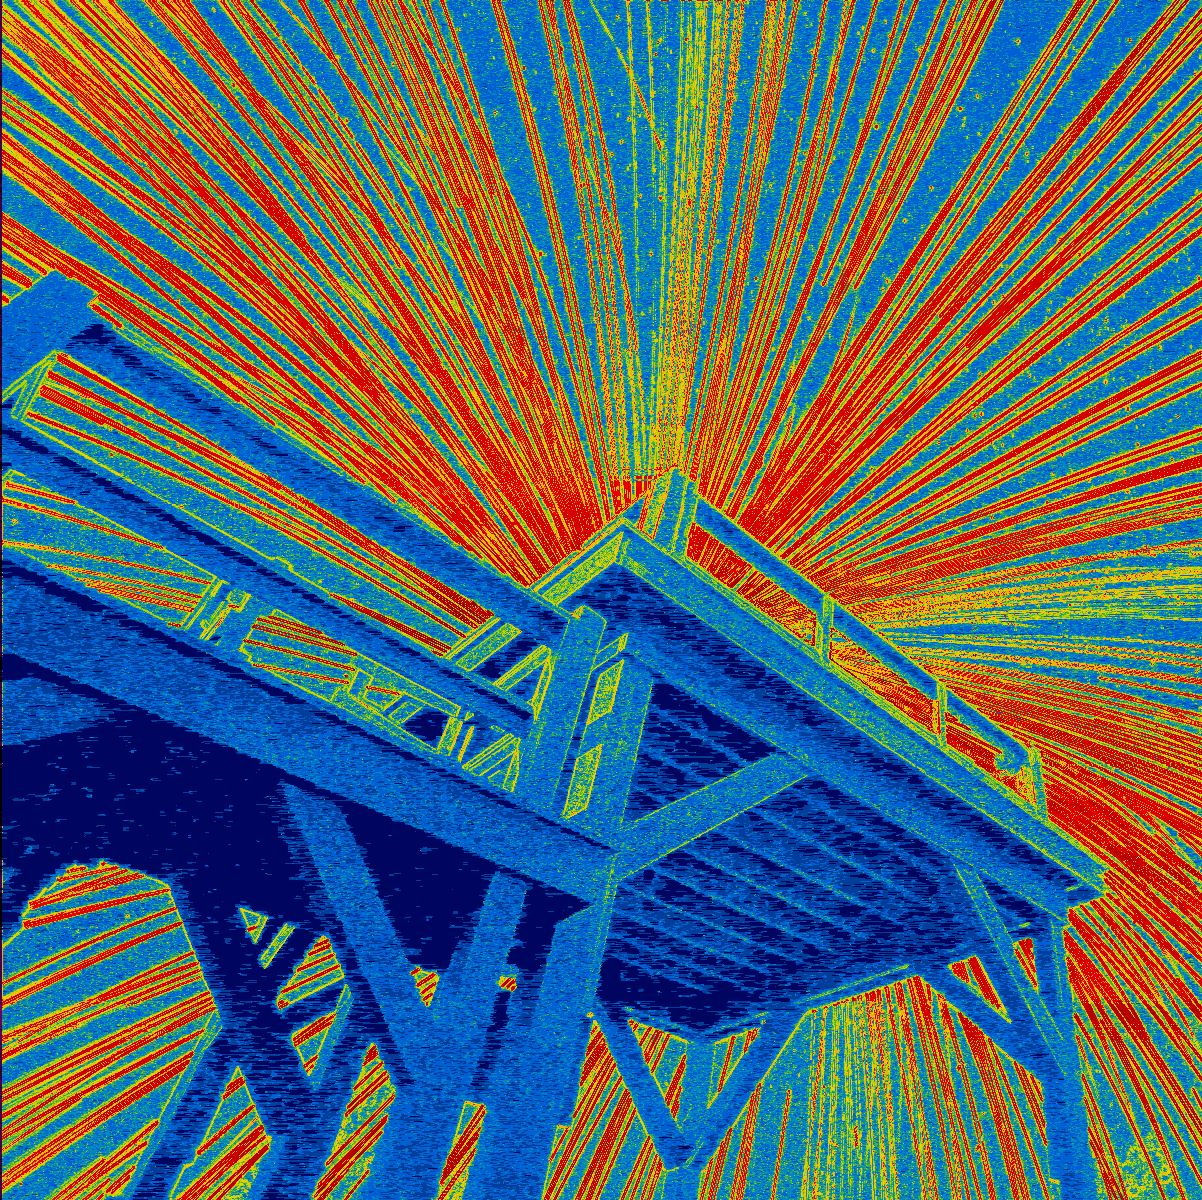
\includegraphics[scale=0.1]{Documeto/1-ElementosTextuais/1-Desenvolvimento/imagens-atividade3/IMG24T.png}

    \fonteElementoGrafico{Adaptado das Fotos Fornecidas pelo Professor}
    
\end{figure}

\paragrafo Outra resultado que nos surpreendeu foi o da imagem 5. Como a foto tratava-se de um reflexo acreditamos que a maior parte da informação seria comprimida, no entanto não foi o suficiente para categorizá-la como baixa. O erro aqui não é necessariamente um julgamento errado, mas sim uma questão de proporção. Nossa análise baseia-se na proporção, como boa parte das partes de menor compressão estavam dispersas pelo cenário a identificação dessa proporção foi prejudicada, culminando no erro.

\begin{figure}[H]
    \centering
    \caption{Visualização da Dificuldade de Compressão da Imagem 5}
    \label{fig:piscina_azul}
    
    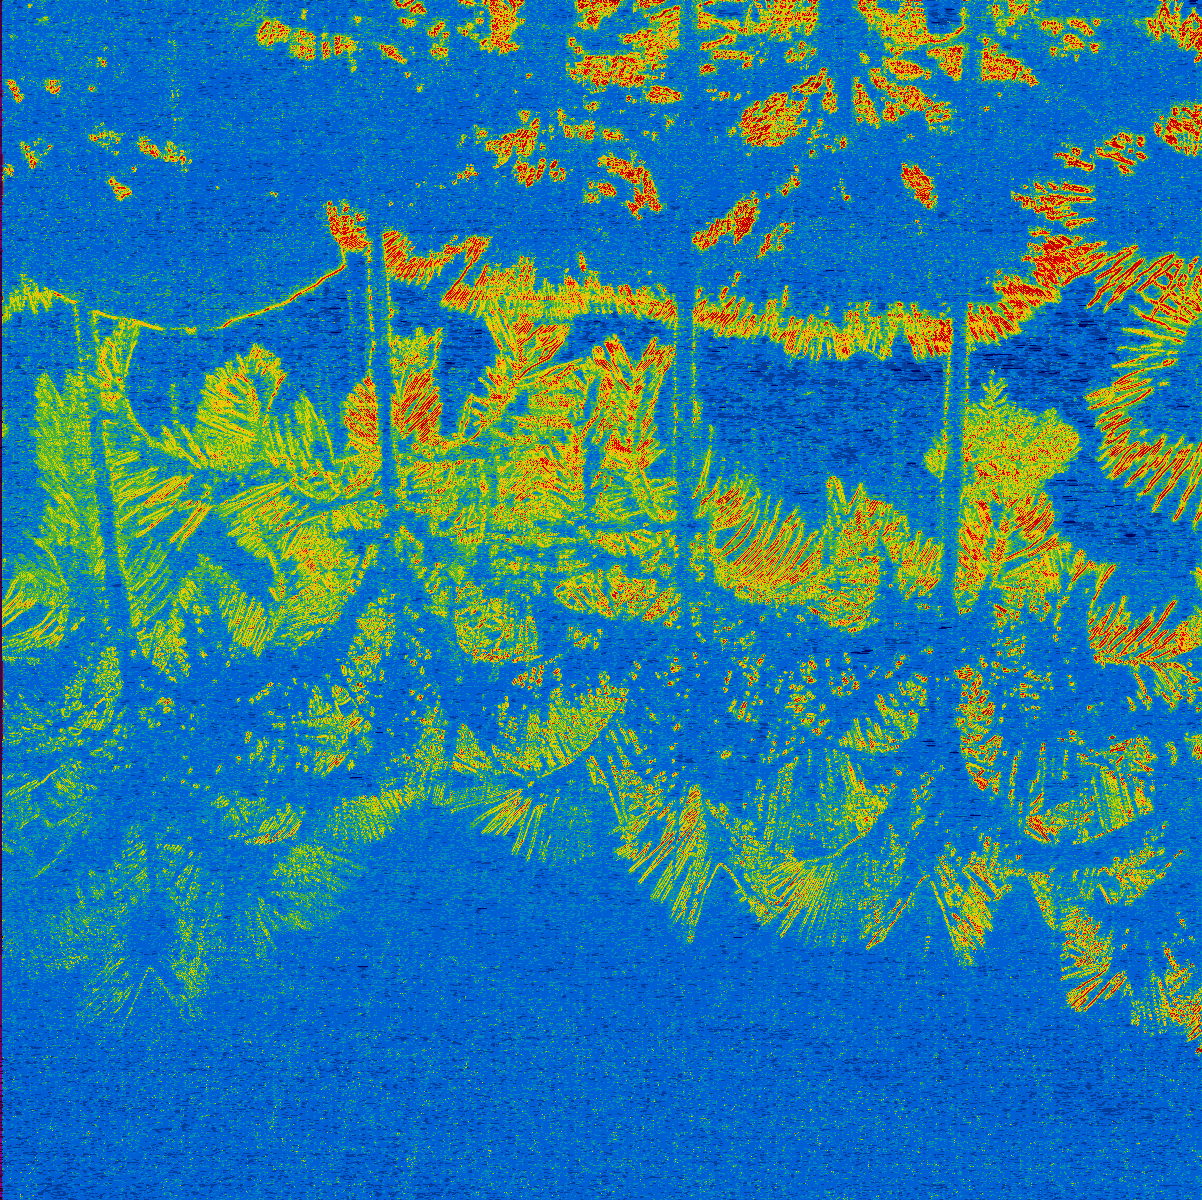
\includegraphics[scale=0.1]{Documeto/1-ElementosTextuais/1-Desenvolvimento/imagens-atividade3/IMG05T.png}

    \fonteElementoGrafico{Adaptado das Fotos Fornecidas pelo Professor}
    
\end{figure}

\paragrafo Também é válido notar como a luz e sombra influenciam na complexidade das informações. Nesse sentido, a imagem 39 é perfeita para expor essa percepção. Acreditamos ser muito difícil que alguém julgue que uma foto de Paris seja julgada como de baixa complexidade. Agora, se perguntarmos onde exatamente ela tem alta complexidade a história muda consideravelmente. 
\begin{figure}[h!]
    \centering
    \caption{Visualização da Dificuldade de Compressão da Imagem 39}
    \label{fig:imagem_39}
    
    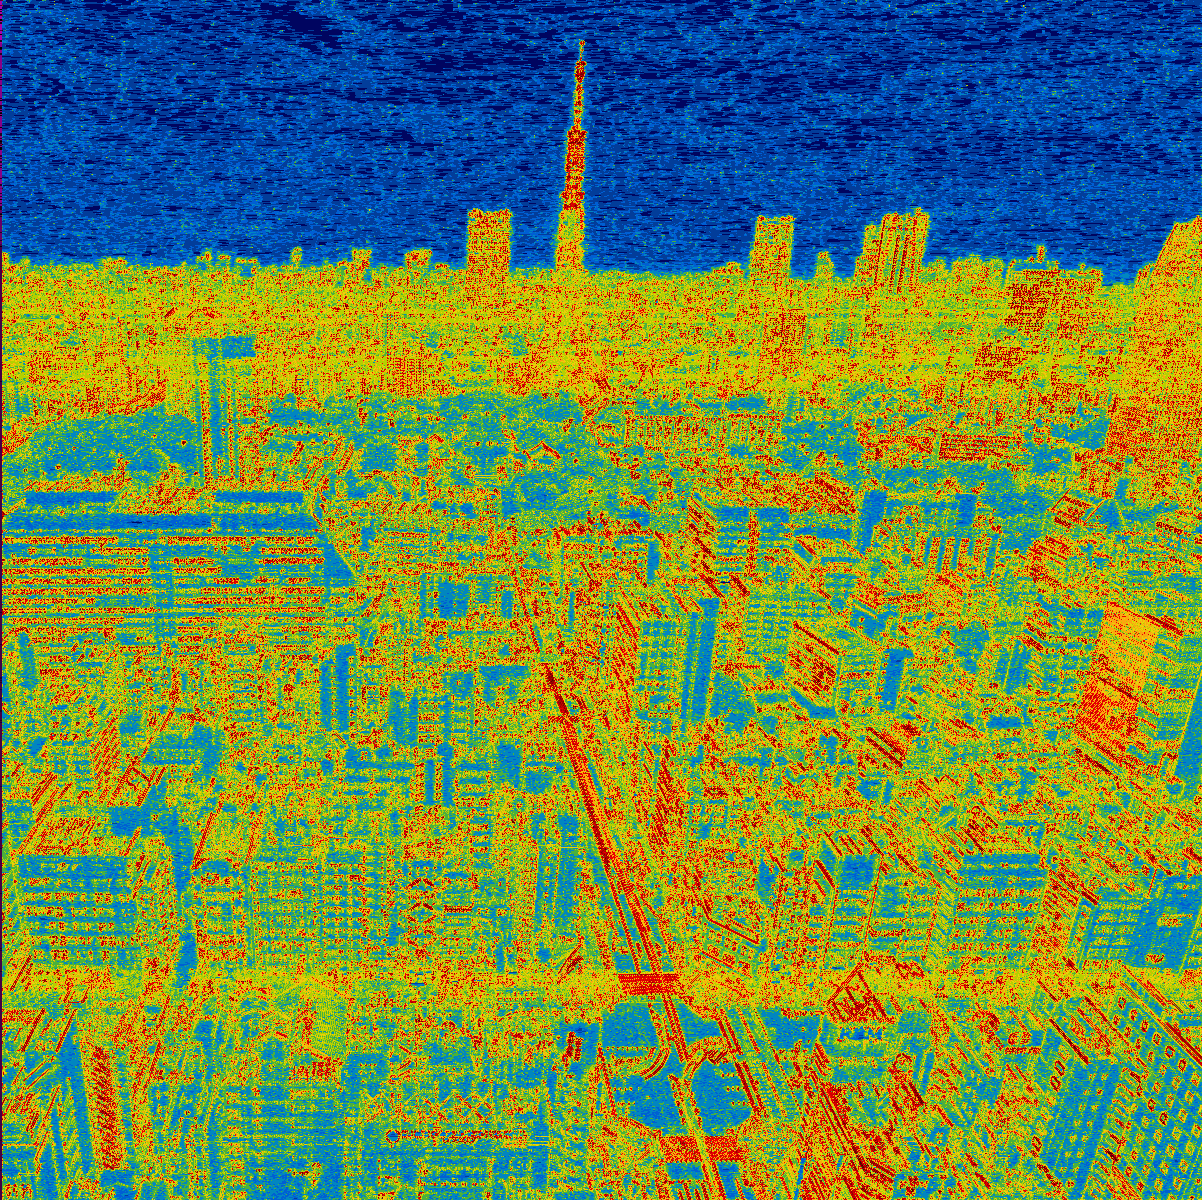
\includegraphics[scale=0.1]{Documeto/1-ElementosTextuais/1-Desenvolvimento/imagens-atividade3/IMG39T.png}

    \fonteElementoGrafico{Adaptado das Fotos Fornecidas pelo Professor}
    
\end{figure}
Se observar a Figura \ref{fig:imagem_39}, de certo notará que as estradas e as paredes dos prédios são facilmente comprimíveis, contudo as janelas, varandas, a própria Torre Eiffel e o ruído gerado p]ela rápida passagem dos carros não são tão bem comprimidas. Isto ocorre porque os focos de luz misturam-se não só entre si bem como em todo o ambiente, aumentando a informação da imagem. Por isso julgamos essa atividade fundamental: julgar a complexidade de imagens é uma coisa, expor onde ela é mais complexa é outro problema completamente diferente.

\newpage
\paragrafo Por fim, decidimos trazer a visualização da compressão da Imagem \ref{fig:imagem_9}. Isso porque ela corrobora com o exposto capítulos antes, mas agora com uma interpretação matemática e mais acurada da situação.


\begin{figure}[h!]
    \centering
    \caption{Visualização da Dificuldade de Compressão da Imagem 09}
    \label{fig:imagem_09}
    
    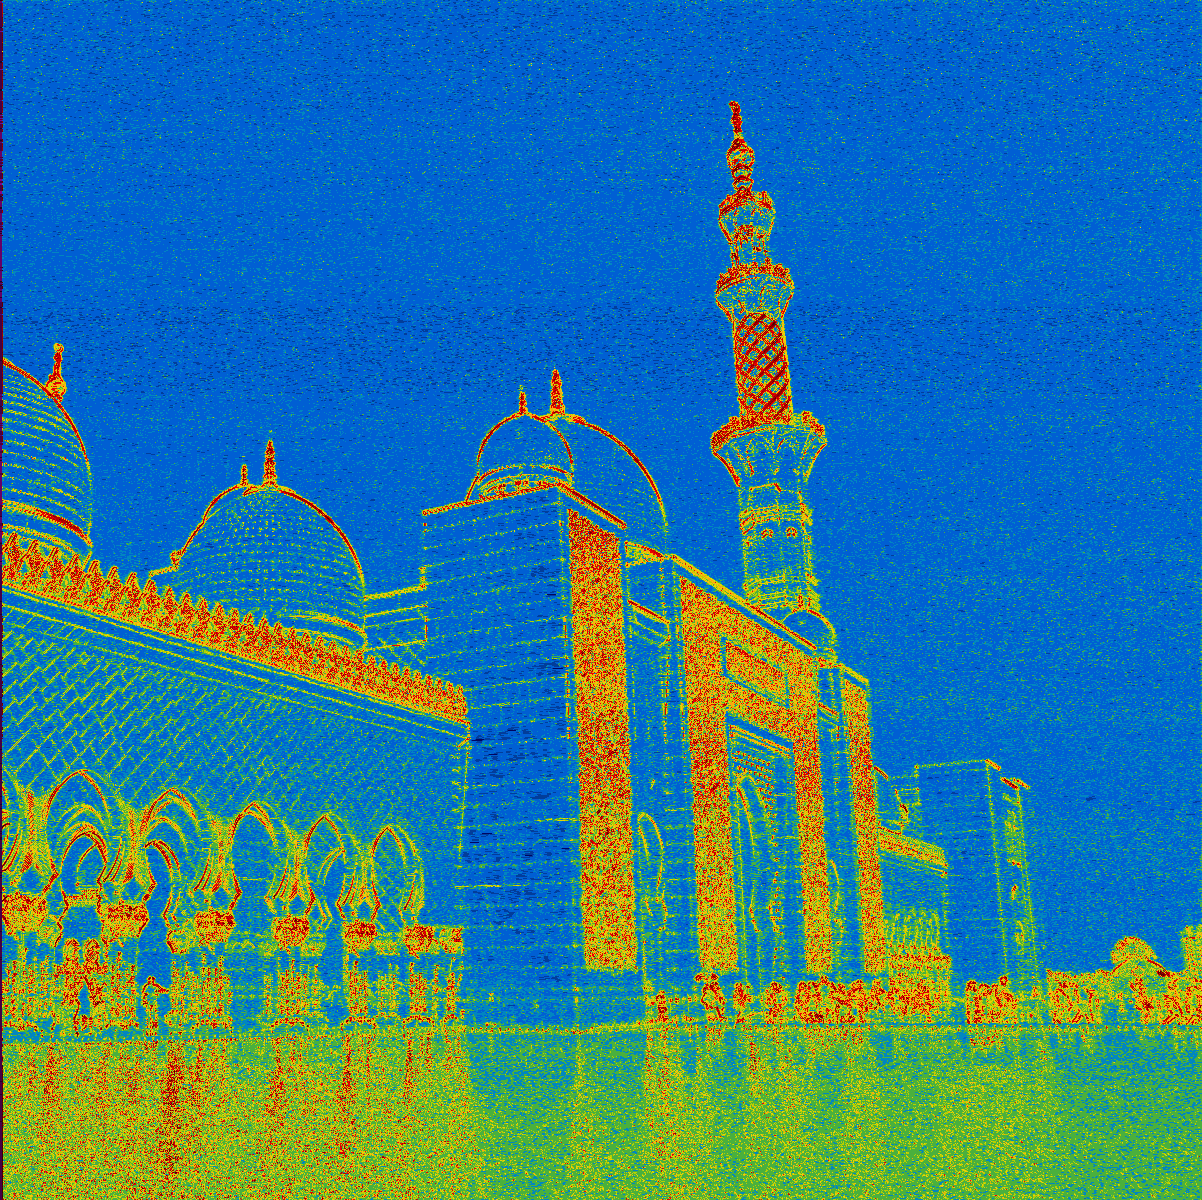
\includegraphics[scale=0.1]{Documeto/1-ElementosTextuais/1-Desenvolvimento/imagens-atividade3/IMG09T.png}

    \fonteElementoGrafico{Adaptado das Fotos Fornecidas pelo Professor}
    
\end{figure}